\chapter{Экспериментальное исследование и анализ результатов}
\label{ch4}

\vspace{0.5cm}

В данной главе представлены результаты экспериментального исследования модифицированного аукционного алгоритма, описанного в главе \ref{ch2}, в сравнении с классическим венгерским алгоритмом. Рассматриваются модельные задачи, имитирующие распределенные системы роботов с различной топологией сети и радиусом связи \( R \). Описываются оценки, включающие количество операций, скорость сходимости, относительную точность. Анализируется эффективность предложенного алгоритма. Результаты визуализированы в виде графиков.

\section{Постановка эксперимента}

\subsection{Модельные задачи}

\vspace{0.3cm}

Для исследования эффективности модифицированного аукционного алгоритма были разработаны модельные задачи, имитирующие распределенные системы роботов. Параметры задач включали:

\begin{itemize}
    \item \textbf{Размер задачи}: Число роботов \( n \) и целей \( m \) варьировалось от 5 до 100, при этом \( n = m \) для сбалансированной задачи.
    \item \textbf{Радиус связи}: Рассматривались значения \( R \in \{10, 20, 30\} \), а также диапазон от 5 до 100 для анализа влияния радиуса на точность.
    \item \textbf{Координаты}: Координаты роботов \( \{p_i = (x_i, y_i)\} \) и целей \( \{q_j = (X_j, Y_j)\} \) генерировались случайным образом в диапазоне \( [0, 100] \) с использованием генератора псевдослучайных чисел.
     \item \textbf{Матрица затрат и выгод}: Затраты \( c_{ij} \) определялись как время, необходимое роботу \( i \) для достижения цели \( j \), вычисляемое по формуле:
    \[
    c_{ij} = \frac{d(p_i, q_j)}{v_i}
    \]
    где \( d(p_i, q_j) \) --- евклидово расстояние между роботом \( i \) и целью \( j \), \( v_i \) --- скорость робота \( i \), предполагаемая постоянной и одинаковой для всех роботов (например, \( v_i = 1 \)). Для решения задачи в терминах максимизации матрица затрат \( c_{ij} \) преобразуется в матрицу выгод \( \alpha_{ij} \) путем вычитания каждого элемента из максимального значения затрат:
    \[
    \alpha_{ij} = C_{\text{max}} - c_{ij}, \quad \text{где} \quad C_{\text{max}} = \max_{i,j} c_{ij}.
    \]
    Задача решается как максимизация суммарной выгоды \( \sum_{i=1}^n \alpha_{i j_i} \), что эквивалентно минимизации суммарного времени \( \sum_{i=1}^n c_{i j_i} \), так как максимизация \( \sum_{i=1}^n (C_{\text{max}} - c_{i j_i}) \) соответствует минимизации \( \sum_{i=1}^n c_{i j_i} \).
    \item \textbf{Матрица связи}: Матрица \( V = \{v_{ij}\} \) формировалась так, что \( v_{ij} = 1 \), если \( d(p_i, p_j) \leq R \), и \( v_{ij} = 0 \) в противном случае.
    \item \textbf{Параметр \( \varepsilon \)}: Для аукционного алгоритма исследовались значения \( \varepsilon \) от \( 10^{-5} \) до 10 с логарифмическим шагом.
\end{itemize}

Каждая задача генерировалась 100 раз для усреднения результатов, что обеспечивало статистическую надежность.

\subsection{Методика проведения экспериментов}

Эксперименты проводились с использованием программной реализации на языке C++ с применением стандартных библиотек для обработки данных и построения графиков. Исследовались следующие аспекты:

\begin{enumerate}
    \item Сравнение количества элементарных арифметических и логических операций, а также обменов между роботами в аукционном и венгерском алгоритмах для различных размеров задачи.
    \item Анализ относительной точности аукционного алгоритма для фиксированных размеров задачи \( n \in \{10, 30, 50\} \) и различных радиусов.
    \item Исследование влияния параметра \( \varepsilon \) на время выполнения и точность при \( n = 80 \) и \( R \in \{10, 20, 30\} \).
    \item Оценка точности аукционного алгоритма на каждой итерации для \( n \in \{10, 30, 50, 100\} \) и \( R = 200 \).
    \item Оценка числа итераций для фиксированного радиуса \( R = 200 \) и различных значений параметра \( \varepsilon \).
\end{enumerate}

Результаты представлены в виде графиков, сохраненных в формате PNG.

\section{Результаты экспериментов}

\subsection{Число операций и обменов}

\vspace{0.3cm}

Эксперименты проводились для \( n = m \) от 5 до 100 и радиуса \( R = 200 \). Результаты представлены на графике (см. рисунок \ref{fig:opeartion_chart}).

\begin{figure}[h]
    \centering
    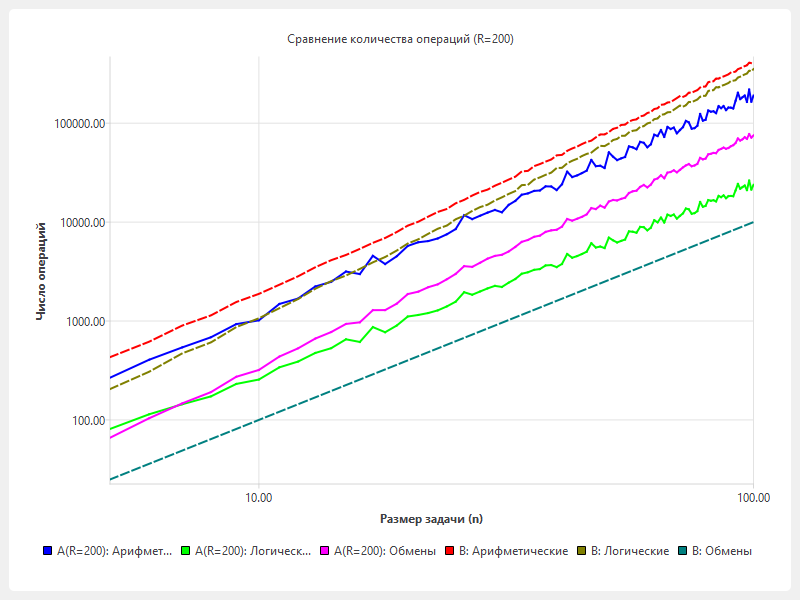
\includegraphics[width=0.8\textwidth]{my_folder/images/operation_chart.png}
    \caption{Зависимость числа операций и обменов аукционного и венгерского алгоритмов от размера задачи.}
    \label{fig:opeartion_chart}
\end{figure}

\vspace{0.3cm}

Эксперименты показывают, что в аукционном алгоритме число арифметических и логических операций значительно меньше, чем в венгерском алгоритме, что делает его более эффективным с точки зрения вычислительной сложности для этих типов операций. Однако число обменов между роботами, которое характеризует количество итераций в аукционном алгоритме, значительно больше, что может замедлять выполнение, особенно при большом числе роботов и целей.

Для повышения эффективности аукционного алгоритма по сравнению с венгерским необходимо, чтобы роботы были оснащены технологиями быстрого обмена данными, обеспечивающими минимальное время передачи информации между собой. Это позволит сократить общее время выполнения алгоритма, сохраняя его преимущества в меньшем числе арифметических и логических операций.

Введение двух характеристик — \( F_{\text{выч}} \) (количество операций в секунду с вещественными или целыми числами) и \( F_{\text{обм}} \) (скорость обмена данными в системе связи, бит/сек) — позволяет оценить, какой подход окажется лучше в зависимости от их значений. Аукционный алгоритм будет предпочтительнее, если \( F_{\text{обм}} \) достаточно высоко, что компенсирует большое число обменов, а \( F_{\text{выч}} \) обеспечивает достаточную вычислительную мощность для обработки меньшего числа операций. Венгерский алгоритм, напротив, будет эффективнее при высоком \( F_{\text{выч}} \) и низком значении \( F_{\text{обм}} \), когда обмены не играют значительной роли из-за централизованного характера алгоритма.



\subsection{Относительная точность}
Точность аукционного алгоритма исследовалась для \( n \in \{10, 30, 50\} \) и \( R \) от 5 до 100 (см. рисунок \ref{fig:accuracy_chart}).

\begin{figure}[h]
    \centering
    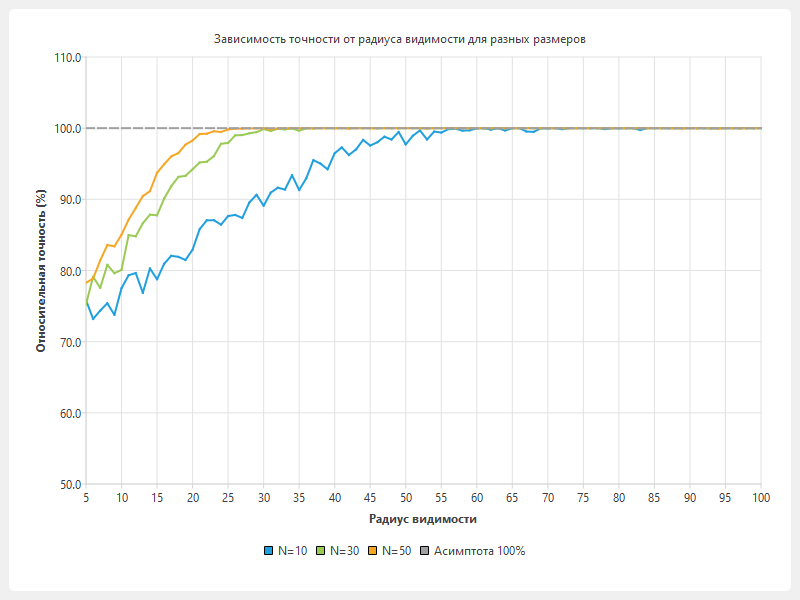
\includegraphics[width=0.8\textwidth]{my_folder/images/accuracy_chart.png}
    \caption{Зависимость относительной точности аукционного алгоритма от радиуса связи для различных размеров задачи.}
    \label{fig:accuracy_chart}
\end{figure}

Выводы:
\begin{itemize}
    \item Точность возрастает с увеличением \( R \), достигая 95--100\% при \( R \geq 50 \).
    \item Для больших \( n \) точность возрастает быстрее из-за меньшего числа связных компонент.
\end{itemize}

\subsection{Влияние параметра \( \varepsilon \)}

\vspace{0.3cm}

Влияние \( \varepsilon \) на время и точность исследовалось для \( n = 80 \) и \( R \in \{10, 20, 30\} \) (см. рисунки \ref{fig:epsilon_time_chart} и \ref{fig:epsilon_accuracy_chart}).

\begin{figure}[h]
    \centering
    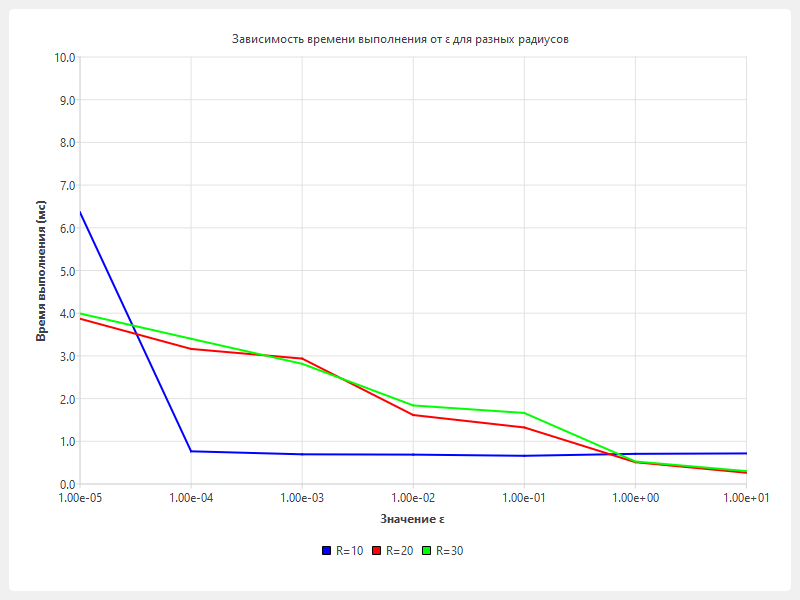
\includegraphics[width=0.8\textwidth]{my_folder/images/epsilon_time_chart.png}
    \caption{Зависимость времени выполнения аукционного алгоритма от \( \varepsilon \) для различных радиусов связи.}
    \label{fig:epsilon_time_chart}
\end{figure}

\begin{figure}[h]
    \centering
    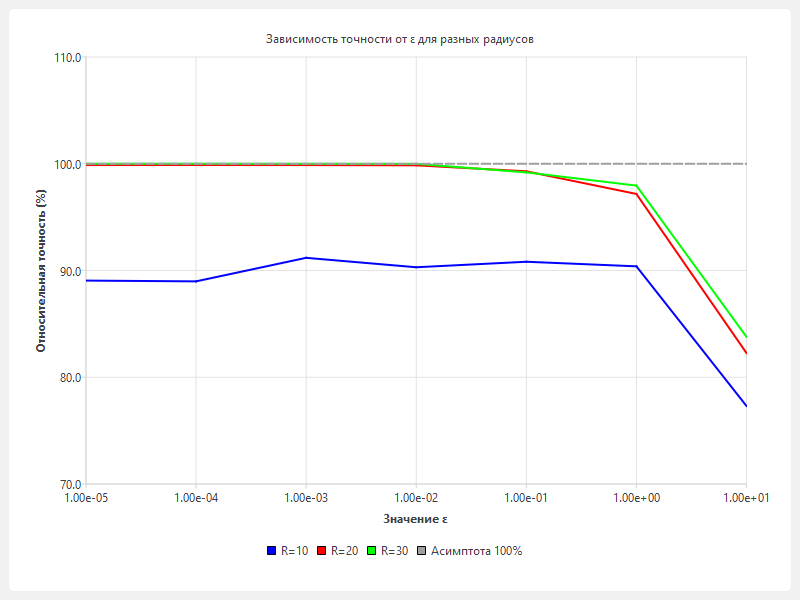
\includegraphics[width=0.8\textwidth]{my_folder/images/epsilon_accuracy_chart.png}
    \caption{Зависимость относительной точности аукционного алгоритма от \( \varepsilon \) для различных радиусов связи.}
    \label{fig:epsilon_accuracy_chart}
\end{figure}

Наблюдения:
\begin{itemize}
    \item Время выполнения уменьшается с ростом \( \varepsilon \), так как требуется меньшее число итераций.
    \item Точность падает при больших \( \varepsilon \), но при \( \varepsilon \leq 10^{-2} \) превышает 90\%.
\end{itemize}

\subsection{Точность по итерациям}

\vspace{0.3cm}

Точность на каждой итерации исследовалась для \( n \in \{10, 30, 50, 100\} \) и \( R = 200 \) (см. рисунок \ref{fig:acc_per_iteration_chart}).

\begin{figure}[h]
    \centering
    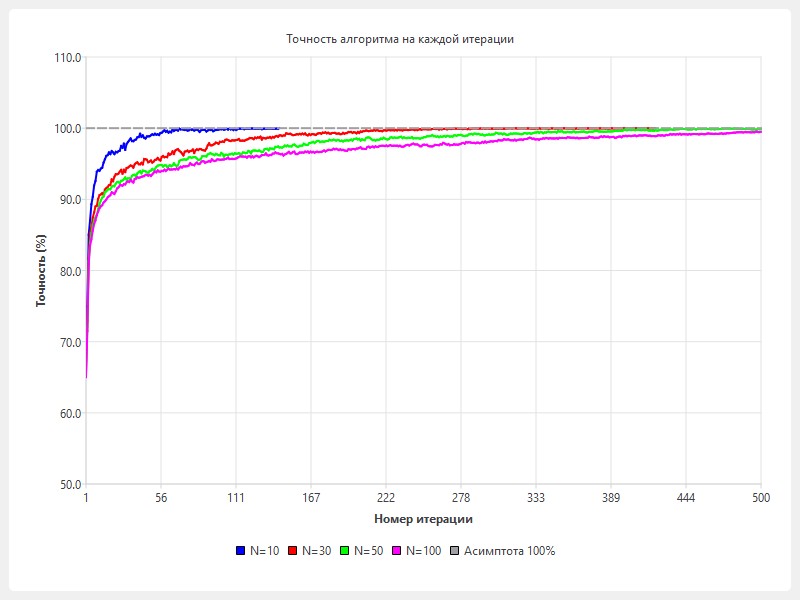
\includegraphics[width=0.8\textwidth]{my_folder/images/accuracy_per_iteration_chart.png}
    \caption{Зависимость относительной точности аукционного алгоритма от номера итерации для различных размеров задачи.}
    \label{fig:acc_per_iteration_chart}
\end{figure}

Наблюдения:
\begin{itemize}
    \item Точность аукционного алгоритма быстро растет на первых итерациях, вплоть до значения относительной точности в 95\%.
    \item Для больших \( n \) требуется больше итераций из-за увеличения числа конфликтов между роботами.
\end{itemize}

\subsection{Количество итераций от заданного параметра \( \varepsilon \)}
\label{sec:iterations_per_epsilon}

Зависимость числа итераций от заданного параметра \( \varepsilon \) исследовалась для \( n \in \{20, 40, 70\} \) и радиуса связи \( R = 200 \) (см. рисунок \ref{fig:iterations_per_acc_chart}). Поскольку матрица выгод \( \alpha_{ij} \) вычисляется на основе матрицы затрат \( c_{ij} \), где \( c_{ij} = \frac{d(p_i, q_j)}{v_i} \), а \( \alpha_{ij} = C_{\text{max}} - c_{ij} \), погрешности измерений расстояний \( d(p_i, q_j) \) влияют на точность \( c_{ij} \) и, следовательно, \( \alpha_{ij} \). Предполагается, что ошибка \( \epsilon_{ij} \) в \( c_{ij} \) подчиняется нормальному распределению \( \epsilon_{ij} \sim N(0, \sigma_c^2) \), где \( \sigma_c^2 \) --- дисперсия ошибки. Соответственно, ошибка в \( \alpha_{ij} \) равна \( \epsilon_{\alpha_{ij}} = -\epsilon_{ij} \sim N(0, \sigma_c^2) \).

Суммарная ошибка целевой функции \( \sum_{i=1}^n \alpha_{i j_i} \) из-за погрешностей измерений равна \( \sum_{i=1}^n \epsilon_{\alpha_{i j_i}} \sim N(0, n \sigma_c^2) \), со стандартным отклонением \( \sqrt{n} \sigma_c \). Согласно теореме \ref{thm:auction_optimality} (глава \ref{ch:analysis}), ошибка аукционного алгоритма ограничена \( n \varepsilon \), следовательно достаточно выбирать \( \varepsilon \) соизмеримым с \( \frac{\sigma_c}{\sqrt{n}} \), чтобы ошибка алгоритма \( n \varepsilon \) была сопоставима с \( \sqrt{n} \sigma_c \). Например, при \( \sigma_c = 0.1 \) и \( n = 40 \), значение \( \varepsilon \) порядка \( 0.0158 \) является подходящим.

 На рисунке \ref{fig:iterations_per_acc_chart} представлена зависимость числа итераций от \( \varepsilon \).

\begin{figure}[h]
    \centering
    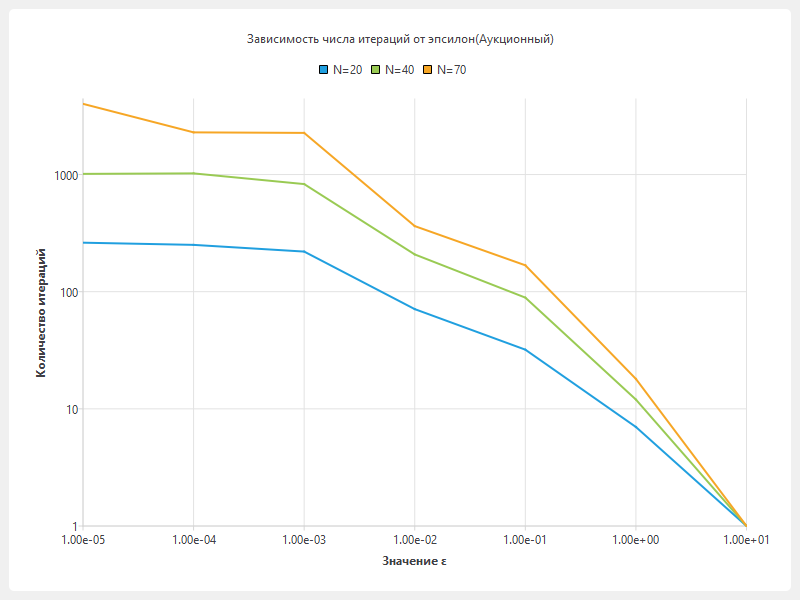
\includegraphics[width=0.8\textwidth]{my_folder/images/iterations_per_accuracy_chart.png}
    \caption{Зависимость числа итераций аукционного алгоритма от параметра \( \varepsilon \) для различных размеров задачи \( n \).}
    \label{fig:iterations_per_acc_chart}
\end{figure}

Наблюдения:
\begin{itemize}
    \item Число итераций монотонно убывает с ростом \( \varepsilon \), что согласуется с теоретической оценкой \( \frac{m \cdot C}{\varepsilon} \).
    \item Для больших \( n \) требуется больше итераций из-за увеличения числа конфликтов между роботами и размера матрицы \( \alpha_{ij} \).
\end{itemize}



\section{Выводы}

Модифицированный аукционный алгоритм продемонстрировал высокую эффективность в задачах распределения ресурсов в системах роботов, обеспечивая баланс между точностью и временем выполнения. Исследования влияния параметров алгоритма, включая радиус связи $ R $, размер задачи $ n $, и параметр $ \varepsilon $, показали, что:
\begin{itemize}
\item Увеличение радиуса связи $ R $ значительно повышает точность алгоритма, достигая 95–100\% при $ R \geq 50 $, особенно для больших $ n $, за счет уменьшения числа связных компонент.
\item Параметр $ \varepsilon $ оказывает существенное влияние на производительность: меньшие значения ($ \varepsilon \leq 10^{-2} $) обеспечивают точность выше 90\%, но увеличивают число итераций, тогда как большие $ \varepsilon $ сокращают время выполнения за счет снижения точности.
\item Параллельная обработка связных компонент снижает вычислительную сложность, делая алгоритм конкурентоспособным по сравнению с классическим венгерским алгоритмом, особенно при высоких скоростях обмена данными ($ F_{\text{обм}} $).
\end{itemize}
Полученные результаты подчеркивают важность настройки параметров аукционного алгоритма для конкретных условий задачи. 